	% Darmstadt|Frankfurt|JuanLesPins
	
	\documentclass{beamer}
	\setbeamertemplate{navigation symbols}{}
	
	\usetheme{hpi}
	\usepackage[ngerman]{babel}
	\usepackage[utf8]{inputenc}
	\usepackage{geometry}
	\usepackage[T1]{fontenc}
	\usepackage{graphicx} %Zum Bilder einbinden
	\usepackage{float} %Damit die Figures, also die Bilder, mitten im Text, an geforceter Position erscheinen
	\usepackage{verbatim} %für mehrzeilige Kommentare \begin~\end{comment}
	\usepackage{amstext} % \text{asdf} in Formeln, statt \mbox, weil mbox die Schriftgröße festsetzt	
	\usepackage{amsmath}
	\usepackage{amssymb}
	\usepackage{ucs}
	\usepackage{BeamerColor}
	
	\usepackage{listings}
	\usepackage{color}
	\usepackage{hyperref}
	\usepackage{acronym}
	\definecolor{tplcolor}{HTML}{F6AE15}
	\usecolortheme[named=tplcolor]{structure}
	
	\lstset{
		language=Java, 
		inputencoding=utf8,
		tabsize=2,
		basicstyle=\tiny,
		captionpos=b,language=JAVA,breaklines=true,      % the size of the fonts that are used for the line-numbers,
		stepnumber=5,   
		keywordstyle=\color{brown},
		commentstyle=\color{DarkGreen}, 
		stringstyle=\color{blue},
		showstringspaces=false,
		breaklines=true
		literate=%
		{Ö}{{\"O}}1
		{Ä}{{\"A}}1
		{Ü}{{\"U}}1
		{ß}{{\ss}}1
		{ü}{{\"u}}1
		{ä}{{\"a}}1
		{ö}{{\"o}}1
		{~}{{\textasciitilde}}1	
	}

	\beamersetuncovermixins{\opaqueness<1>{25}}{\opaqueness<2->{15}}
	
	\usecaptiontemplate{
	\tiny
	\structure{\insertcaptionname~\insertcaptionnumber:}
	\insertcaption
	}
	
	\usefootnotetemplate{
	\tiny
	\parindent 1em\noindent
	\hbox to 1.8em{\hfil\insertfootnotemark}\insertfootnotetext
	}
	\begin{document}
			
	\setbeamercovered{invisible}
	
	\title[Review - Analyseprojekt]{Review - Analyseprojekt\\ Eine Mitgliederverwaltung für den Malteser Hilfsdienst}
	\author{Gruppe 3}
	
	 \begin{frame}[title=Hauptgebaeude_Nacht.jpg]
	 \maketitle
	 \date{22. Mai 2018}
 	\end{frame}
	 
	\begin{frame}
		\frametitle{Gliederung}
		\tableofcontents
		%Folien mit einem * im Titel sollen beim Vortrag übersprungen werden.
	\end{frame}

\section{Produkteinsatz}		
\begin{frame}
\frametitle{Produkteinsatz}
Im Folgenden werden die notwendigen Fachbegriffe und Zusammenhänge näher erläutert. Des Weiteren werden systemrelevante Abläufe im Einsatzbereich dargestellt und die erläuterten Fachbegriffe in Beziehung zu diesen Abläufen gesetzt.\\
Dafür wird bewusst ein IST-Zustand der aktuellen Situation aufgeführt, um daraus den Einsatz des neuen Produktes (SOLL-Zustand) herzuleiten.
\end{frame}

\subsection{Beschreibung des Problembereichs}		
\begin{frame}
\frametitle{Beschreibung des Problembereichs}
Im Rahmen der Aufgabenstellung wird hier auf eine Problembereichs-Beschreibung verzichtet. Allerdings sind folgende Annahmen über den Problembereich getroffen worden:
\begin{itemize}
\item Stammdaten können geändert werden, allerdings sind manche dieser Daten (z.B. E-Mail-Adresse) bei einer Änderung zu verifizieren. Andere wiederum können ohne Verifizierung direkt geändert werden.
\item Einsatzleiterausbildungen sind Qualifikationen, auch wenn sie im gegebenen Beispiel als eigene Spalte aufgeführt werden.
\item Fähigkeiten eines Helfers, die nicht urkundlich nachgewiesen werden müssen, werden nicht in der Personalverwaltung aufgeführt
\end{itemize}
\end{frame}

\subsection{Glossar}		
\begin{frame}
\frametitle{Glossar}
\begin{acronym}[Qualifikation]  
\acro{Stammdaten}{Personenbezogene und persönliche Daten, die direkt beim Eintritt erfasst werden. Diese umfassen Namen, Vornamen, Geburtsdaten, Adresse, Telefon, Mailadresse und evtl. Bankdaten des jeweiligen Helfers.} 
\acro{Helfer}{Synonym zu Ehrenamtlicher, alle erfassten Mitglieder, die nicht hauptamtlich tätig sind. Bezieht sich nicht auf die Fähigkeit, an Sanitätseinsätzen o.Ä. teilnehmen zu können.}  

\end{acronym}
\end{frame}

\begin{frame}
\frametitle{Glossar}
\begin{acronym}[Führungskraft]  
	\acro{Qualifikation}{Urkundlich nachweisbare Befähigung eines Helfers. Diese Befähigung kann einerseits den Helfer zu mehr Aufgabenbereichen befähigen (wie dem Führen eines Fahrzeugs), andererseits auch verpflichtend sein, um weiterhin Helfer zu sein (wie die Arbeitsmedizinische Untersuchung). Qualifikationen können unbefristet gültig sein, sie können aber auch nach einer gewissen Dauer ablaufen und müssen danach erneut nachgewiesen werden (z.B. Führerschein).
	}
	\acro{Führungskraft}{Helfer, die eine von den fünf Rollen Personalbeauftragter, Neuhelferbeauftragter,
		Ausbildungsbeauftragter, Einsatzkoordinator und Fahrzeugbeauftragter übernommen haben. Ein Helfer kann jeweils höchstens eine solche Funktion übernehmen.}  
\end{acronym}
\end{frame}
\subsection{Modell des Problembereichs}		
\begin{frame}
\frametitle{Modell des Problembereichs - IST}
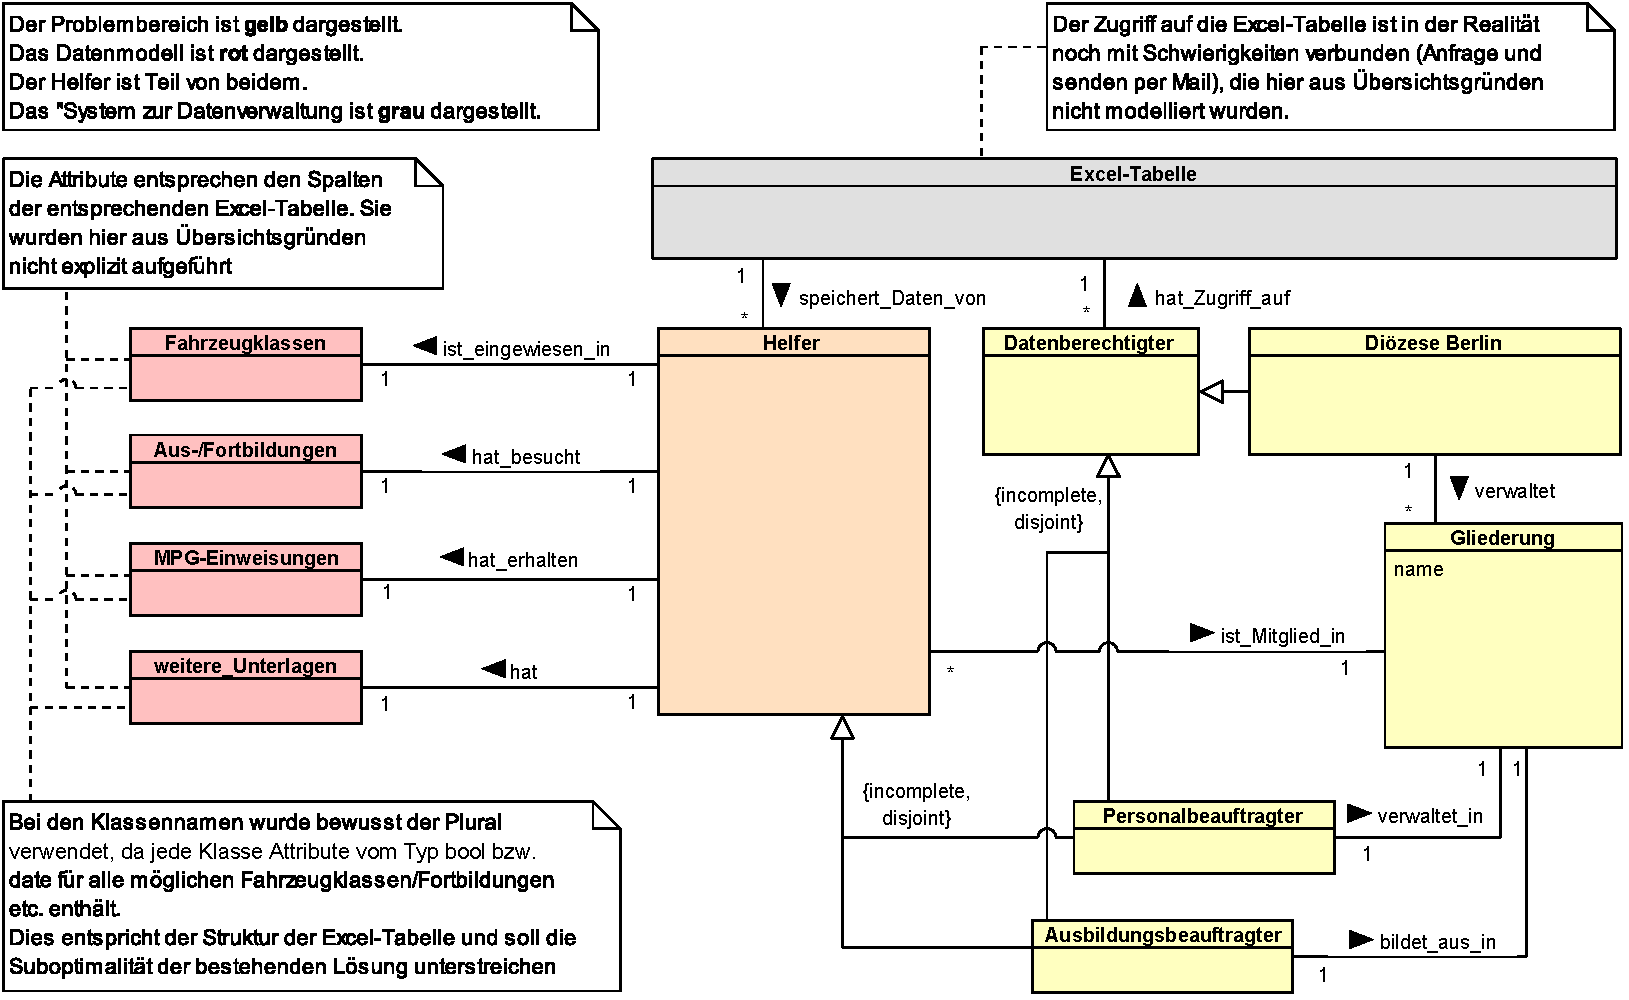
\includegraphics[height=0.75\textheight]{PDF/Klassendiagramm_ist.pdf}
\end{frame}
\begin{frame}
\frametitle{Modell des Problembereichs - SOLL}
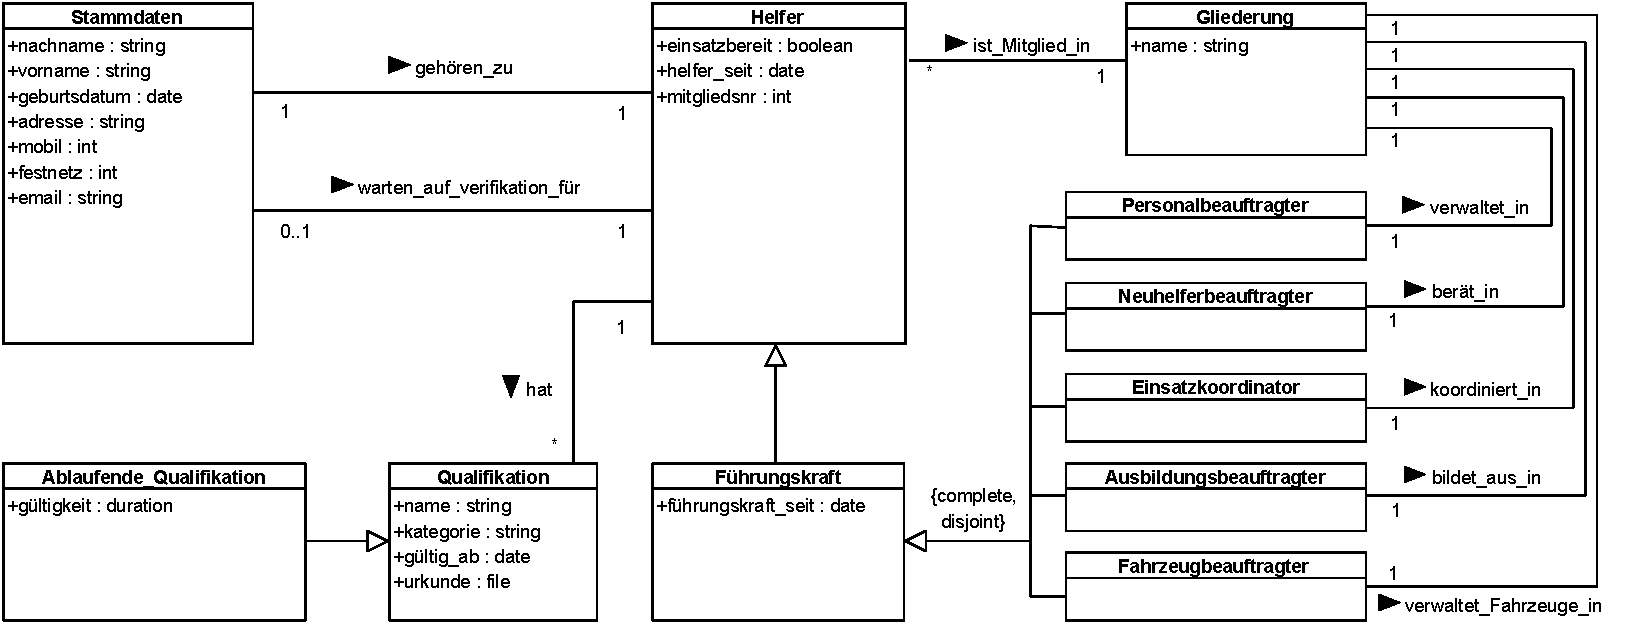
\includegraphics[width=\textwidth]{PDF/Klassendiagramm_soll.pdf}
\end{frame}

\subsection{Geschäftsprozesse}		
\begin{frame}
\frametitle{Den Maltesern beitreten}
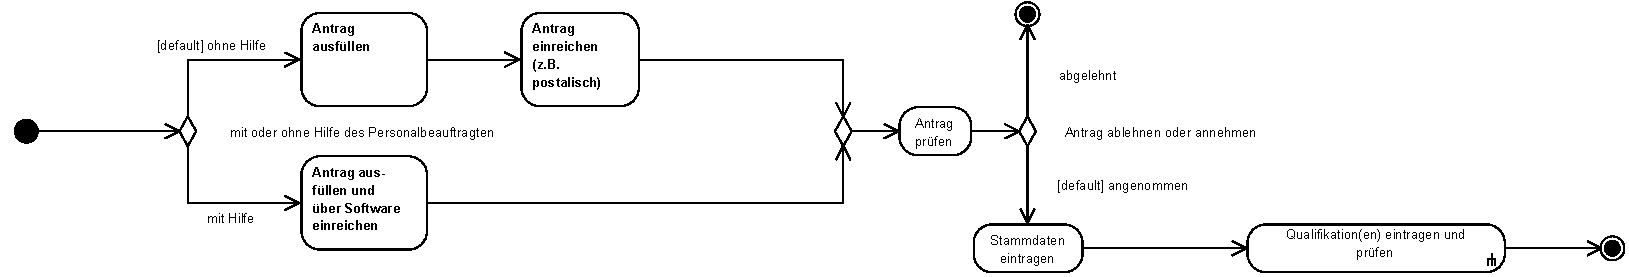
\includegraphics[width=\textwidth]{PDF/BusinessP/Mitglied_werden.pdf}
\textbf{Anmerkung: } Grau markierte Aktivitäten und Aktionen stellen menschliche Interaktionen mit dem System dar.
Wenn ein Außenstehender beschließt, den Maltesern beizutreten, so füllt dieser evtl. mit Beteiligung des Neuhelferbeauftragten einen Antrag aus, welcher von der Diozöse bearbeitet wird. Das Ergebnis ist dann entweder eine Antragsablehnung oder die Eintragung der Stammdaten des Antragsstellers, was einem Beitritt entspricht. 
\end{frame}
\begin{frame}
\frametitle{Helferdaten abrufen}
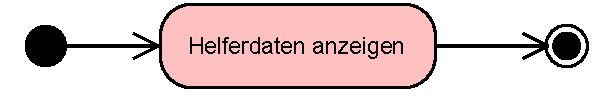
\includegraphics[width=\textwidth]{PDF/BusinessP/Daten_abrufen.pdf}
Wer dazu berechtigt ist (z.B. Personalbeauftragter), kann die für ihn freigegebenen Daten der für ihn sichtbaren Helfer einsehen.
\end{frame}

\begin{frame}
\frametitle{Personenbezogene Daten ändern}
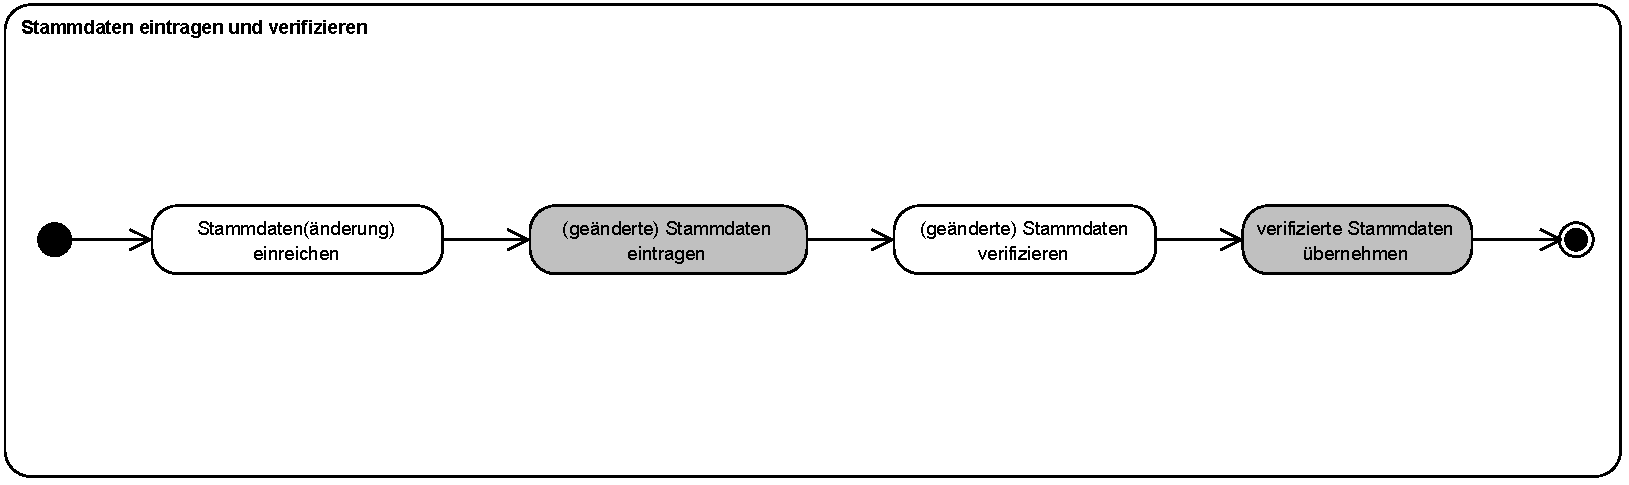
\includegraphics[width=\textwidth]{PDF/BusinessP/Daten_aendern.pdf}
Sollen Änderungen an Stammdaten eines Helfers vorgenommen werden, so reicht selbiger Helfer diese Änderungen beim Personalbeauftragten ein, welcher die Änderungen vornimmt. Betrifft die Änderung zu verifizierende Daten, so muss außerdem die Diozöse selbige verifizieren.
\end{frame}

\begin{frame}
\frametitle{Qualifikation eintragen}
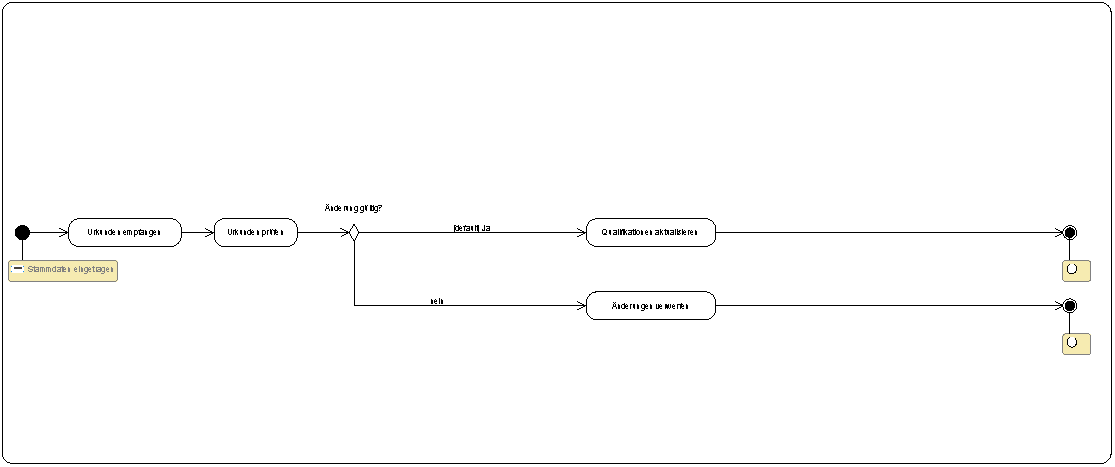
\includegraphics[width=\textwidth]{PDF/BusinessP/Qualifikation_eintragen.pdf}
Erwirbt ein Helfer eine neue Qualifikation oder muss die Verlängerung einer Bestehenden nachweisen, dann reicht er die zugehörige Urkunde ein.\\
Der Personalbeauftragte prüft ggf. unter Rücksprache mit dem Ausbildungsbeauftragten die Gültigkeit der Urkunde und trägt nachgewiesene Qualifikationen ein.
\end{frame}


\begin{frame}
\frametitle{Ablaufende Qualifikation erneuern}
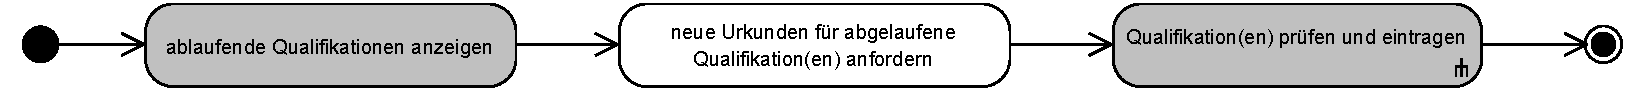
\includegraphics[width=\textwidth]{PDF/BusinessP/Qualifikation_erneuern.pdf}
Personalbeauftragte und Ausbildungsbeauftragte können sich die Qualifikationen der für sie sichtbaren Helfer, die bald ihre Gültigkeit verlieren, anzeigen lassen und danach die betreffenden Helfer an die Einreichung aktueller Urkunden / Nachweise erinnern.
\end{frame}

\begin{frame}
\frametitle{Aus den Maltesern austreten}
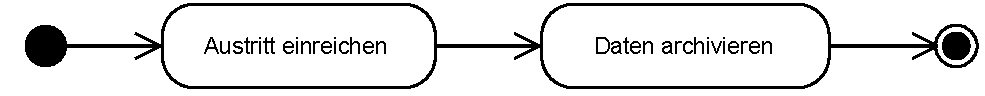
\includegraphics[width=\textwidth]{PDF/BusinessP/Austreten.pdf}
Wenn ein Mitglied beschließt, die Malteser zu verlassen, reicht es seinen Antrag beim Personalbeauftragten ein, welcher infolgedessen die gesamten Daten des Mitglieds archiviert.
\end{frame}


\section{Produktfunktion}		
\begin{frame}
\frametitle{Produktfunktion}
\begin{minipage}{0.6 \textwidth}
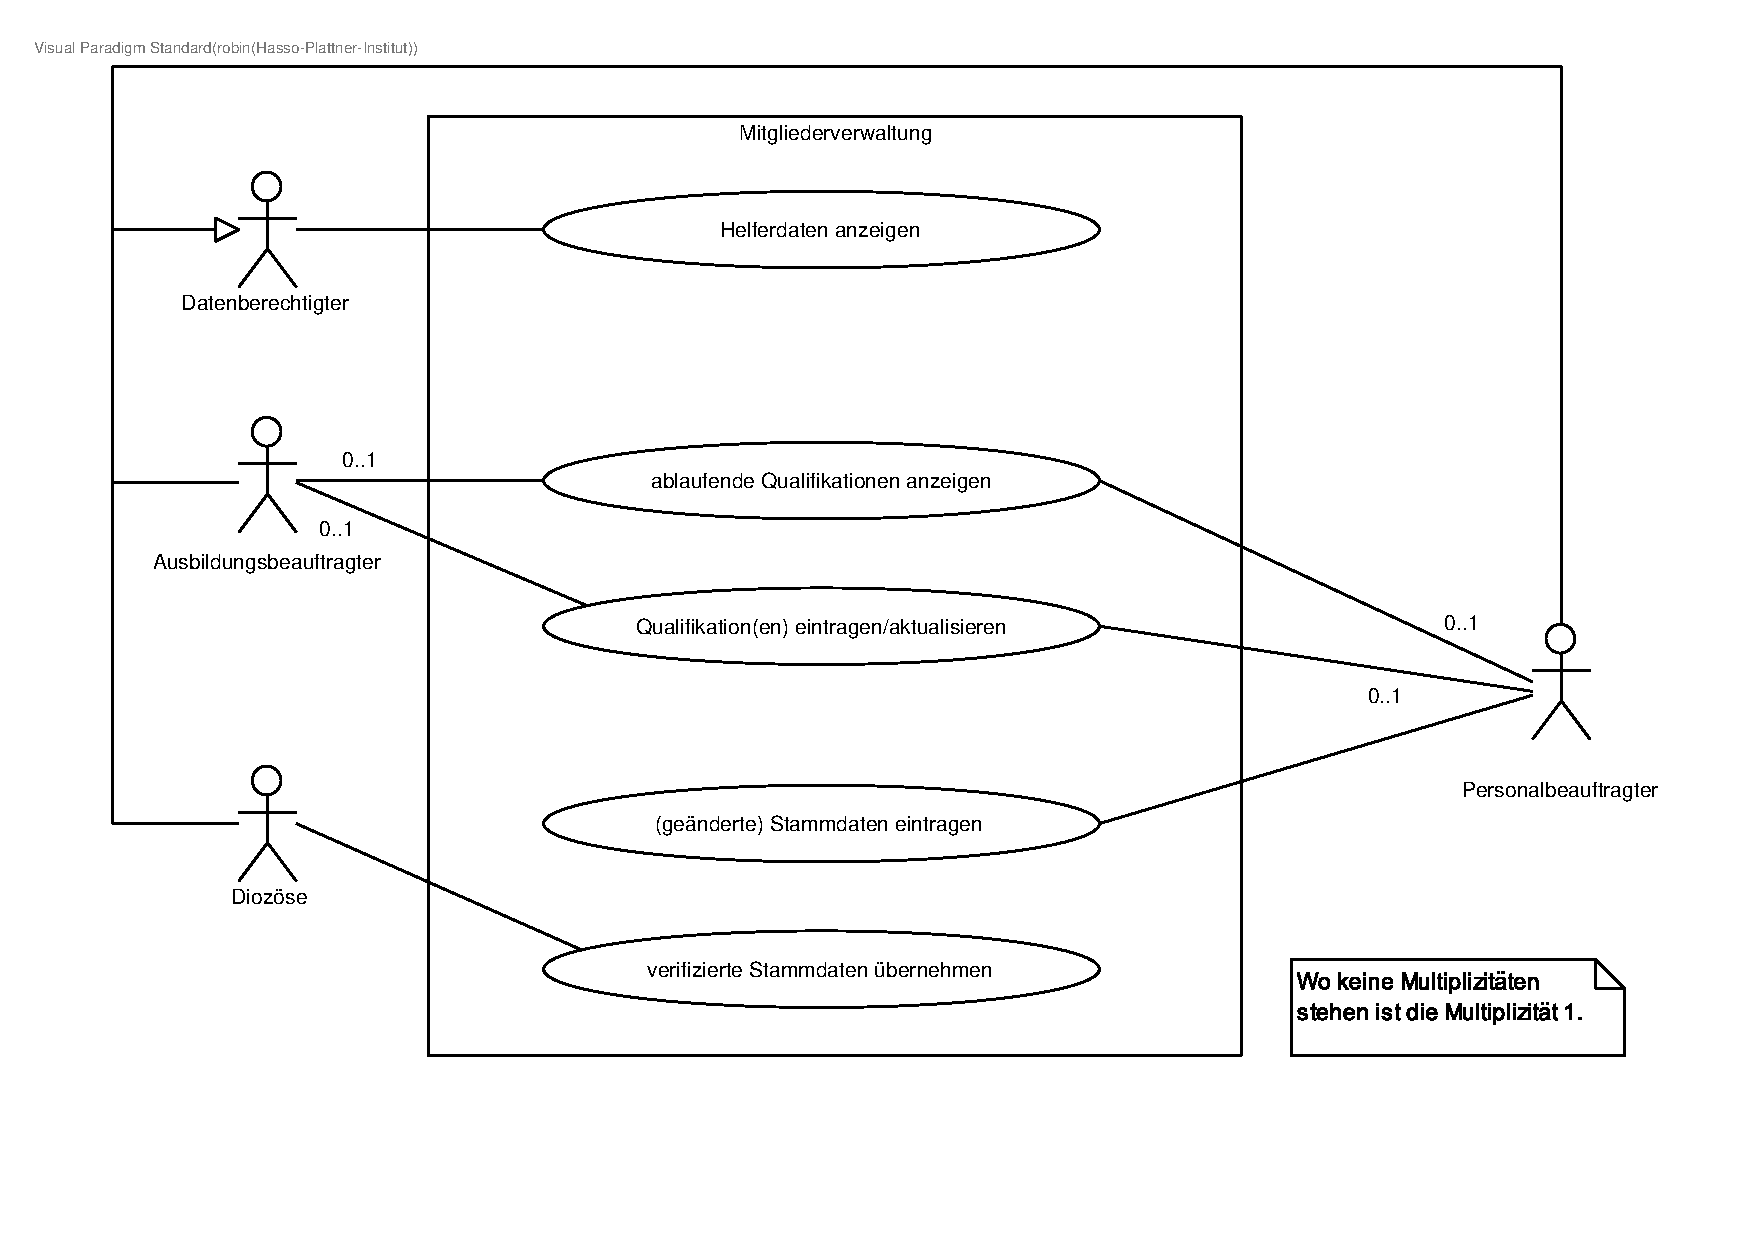
\includegraphics[height=0.75 \textheight]{PDF/Use_Case.pdf}
\end{minipage}
\hfill
\begin{minipage}{0.3 \textwidth}
	Da die dargestellten Use Cases sich eng an die vorher definierten Geschäftsprozesse anlehnen, wurde auf die separate Modellierung eines Use Cases als Geschäftsprozess im folgenden Abschnitt verzichtet.
\end{minipage}
\end{frame}

\subsection{Anwendungsfälle im Überblick}		
\begin{frame}
\frametitle{Anwendungsfälle im Überblick}
\begin{acronym}[Qualifikation(en) eintragen/aktualisieren]
	\acro{Helferdaten anzeigen} {Berechtigte Personen (z.B. Personalbeauftragter der Gliederung, hauptamtliche Mitglieder der Diozöse) können die für sie freigegebenen Helferdaten abrufen.}
	\acro{ablaufende Qualifikationen anzeigen} {Berechtigte (z.B. Personalbeauftragte) können sich anzeigen lassen, welche Qualifikationen (z.B. Führerscheine) bald nicht mehr gültig sind.}
		\acro{Qualifikation(en) eintragen/aktualisieren} {Wird eine neue Qualifikation wie eine neue Führerscheinklasse erworben oder eine bestehende Qualifikation verlängert, wird die zugehörige Urkunde geprüft und die Qualifikation eingespeichert.}
	\end{acronym}
\end{frame}



\begin{frame}
\frametitle{Anwendungsfälle im Überblick}
\begin{acronym}[verifizierte Stammdaten übernehmen]
	\acro{(geänderte) Stammdaten eintragen}{Ändern sich die Stammdaten eines Helfers (wie Adresse, Telefonnummer, ...) teilt dieser das dem Personalbeauftragten mit, welcher die gespeicherten Daten aktualisiert.}
	\acro{verifizierte Stammdaten übernehmen} {Manche Stammdatenänderungen (wie Telefonnummer) müssen verifiziert werden, bevor das System sie übernimmt. Die hauptamtlichen Mitarbeiter der Diozöse führen die entsprechenden Prüfungen durch und tragen sie nach Bestätigung ein.}
\end{acronym}
\end{frame}

\begin{frame}
\frametitle{Anwendungsfälle im Überblick}
\begin{acronym}[Helferdaten archivieren]
	\acro{Helfereintrag anlegen}{Tritt ein neues Mitglied bei, werden dessen Stammdaten entweder direkt vom Neuhelferbeauftragten beim persönlichen Gespräch oder nach Aufnahmeinformation von der Bundesverwaltung ins System eingegeben.}
	\acro{Helferdaten archivieren} {Tritt ein Mitglied aus den Maltesern aus, werden dessen Stamm- und Qualifikationsdaten in einer separaten Datenbank gespeichert und können bei einem erneuten Beitritt wieder geladen werden.}
\end{acronym}
\end{frame}

\begin{frame}[title=Hauptgebaeude_Nacht.jpg]
\maketitle
\date{22. Mai 2018}
\end{frame}
\end{document}

